\documentclass{article}
\usepackage{times}
\usepackage{cite}
\usepackage[margin = 1in]{geometry}
\usepackage{amsfonts, amsmath, amssymb}
\usepackage[none]{hyphenat}
\usepackage{fancyhdr}
\usepackage{listings}
\usepackage[nottoc,notlot,notlof]{tocbibind}
\usepackage{amsmath}  % for \text macro
\usepackage{amssymb}  % for \mathbb macro
\usepackage{graphicx}
\usepackage[spaces,hyphens]{url}
\usepackage[utf8]{inputenc}


\newtheorem{theorem}{Theorem}
\newenvironment{proof}{\noindent{\bf Proof:}}{$\hfill \Box$ \vspace{10pt}}  
\pagestyle{fancy}
\fancyhead{}
\fancyfoot{}
\fancyhead[L]{\slshape \MakeUppercase{Final year project}}
\fancyhead[R]{\slshape Feasibility Report}
\fancyhead[C]{\thepage}
\renewcommand{\footrulewidth}{0pt}
\parindent 0ex
\setlength{\parindent}{4em}
\setlength{\parskip}{1em}
\renewcommand{\baselinestretch}{1.5}
\begin{document}
\begin{titlepage}
\begin{center}
\vspace*{1cm}
\begin{figure}[h!]
\centering

\includegraphics[scale=0.5]{logo}
\end{figure}
\Large\textbf{Feasibility Report}\\
\Large\textbf{Final Year Project}\\
\vfill
\line(1,0){400}\\[1mm]
\huge{\textbf{SmartGuide: A smart campus guide using BLE based indoor localization}}\\[3mm]
\line(1,0){400}\\
\vfill

\large{Tooba Naseer  (2016-CE-72)}\\
\large{Rida Mahmood  (2016-CE-54)}\\
\large{Ayesha Jabbar  (2016-CS-159)}\\
\large{Rabeya Hamood  (2016-CE-81)}\\
\large{Supervised by: Dr. Sheikh Faisal Rasheed}\\
\large{Co-advisor : Dr. Beenish Ayesha Akram}\\
\large{\textbf{Department of Computer Science and Engineering}}\\
\large{\textbf{University of Engineering and Technology, Lahore}}\\
\end{center}
\end{titlepage}
\tableofcontents
\thispagestyle{empty}
\clearpage
\setcounter{page}{1}

\makeatletter
\newcommand{\heading}[1]% #1 = text
{\par\vskip 1.5ex \@plus .2ex
 \hangindent=1em
 \noindent\makebox[1em][l]{$\,\bullet$}\textbf{\large #1}%
\par\vskip 1.5ex \@plus .2ex
\@afterheading}
\makeatother

\section{Introduction}

\subsection{Overview of Project}
Outdoor and indoor localization is an integral component of  IoT (Internet of Things) in this era of mobile computing. Indoor localization can open new horizons for ubiquitous applications targeting university departments, government small institutes, software houses, airports, shopping malls, museums etc. Our project will find the location of a specific person by using appropriate machine learning approach using BLE based Android application. This location will be used to provide guided tour of the indoor building (Computer Science and Engineering Department at UET, Lahore) we will use to validate our work. 
\\\\
This project will guide persons who are not much familiar with visiting place. It has an android application that will predict the indoor location of a person at room level and also gives information of current room location and nearby rooms in the form of text, images, audio and videos. In our case visiting place will be CSE dept at UET LHR. For room prediction, RSSI fingerprints of BLE beacons will be captured for training of model. After finding the location of the person, guidelines of that certain room/area will be provided to the user on user end android application. Indoor positioning has numerous applications. We can use indoor positioning of people to guide them inside shopping malls, airports or museums. 



\subsection{Background}
Outdoor localization has been formalized by using satellite-based technologies i.e. GPS\cite{GPS}, BeiDou\cite{cooper2016loco}, GLONASS\cite{cooper2016loco}, and GALILEO\cite{GALILEO}. It is hard for finding the indoor location by using conventional GPS technology because of no direct (Line of Sight)\cite{akram2018censloc} in indoors, so we cannot use these technologies for indoor positioning. Up to date, the technologies used for indoor localization approach are: TOA (Time of Arrival), TDOA (Time Difference of Arrival), AOA (angle of arrival) but they have some limitations. TOA and TDOA require precise clock count and its synchronization and AOA-based systems require special antennas for their propagation. So, we are going to implement a system which employs suitable machine learning approach to find the location by using RSSI (Received Signal Strength Indicator) fingerprinting technique. This RSSI values will pass to the trained model (a model which is trained on a given set of input and output values by using appropriate machine learning algorithm) which gives the location of the mobile device.
\subsection{Motivation}
People/visitors who go to an unknown place find it difficult to traverse and wants to find places/people of interest easily. Such problems motivate us to provide ease and leverage facility to users so that they can see the information of a particular indoor environment on his mobile application automatically. BLE is available on nearly every smart device so no additional hardware required at user end. Hence by utilizing their indoor location determined using machine learning on BLE fingerprints, guided tours of smart campus to visitors can be provided and facilitating them. We are using latest technology of BLE beacons because they work on battery and consume less energy than Wi-Fi signals\cite{hultgren2015evaluating}.
\section{Goal of the project}
The main target user of our system is a visitor of a university campus. So, our goal is to provide ease and guidance to him regarding a particular lab and its nearby labs automatically via installed application on device by estimating his indoor location. The guidance involves the textual and pictorial information about that particular indoor environment.
\section{Objectives of the project}
\subsection{Industry Objectives}
\begin{itemize}
\item Implement a system that takes into account the demands of university campus exploration.
\item This project leads to visitors of any organization or store to save their time and effort by providing them textual and pictorial information of organization or store.
\item Industrial administrators seek advantage of their time by providing much information to their customers in less time which automatically increase the sales and profit of their product.
\item To provide the solutions of the problems that people are facing while they visit first time to a certain campus.


\end{itemize}
\subsection{Research Objectives}
\begin{itemize}
\item To find the location of the user that will be connected to his android app via Bluetooth technology\cite{Introduction}.
\item To monitor and provide guidelines to user who is connected to the BLE beacon via Bluetooth and mobile application, we need to find user location inside buildings.
\item To develop an android application which provide textual and pictorial information of particular area and its nearby areas to the user who is located in that indoor environment.


\end{itemize}
\subsection{Academic Objectives}
\begin{itemize}
\item This project enables us to understand the concepts of following subjects:
\\a.	Machine learning
\\b.	Networking
\\c.	Android development
\\d.	Front-end design
\\e.	Client server communication management
\item To complete a whole real world project , utilizing concepts from computer networking, databases, machine learning, software development life cycle of SE , testing and mobile development.
\item To develop the understanding and connection between the android app and the hardware structure. 
\item To find the best Machine Learning algorithms which are used to train the model of fingerprints. 
\item To make an android application which use as an interface to provide guidelines to the user who is located in a particular indoor environment.
\item To ensure the use of latest technologies in implementing the project which helps technical persons and students to enhance their academic skills via learning new features


\end{itemize}

\section{Scope of the project}
In this project, android application runs on a user’s mobile device and and will capture BLE RSSI fingerprints. The fingerprints collected at the initial stage will be processed and used to train suitable machine learning model, after training of the ML based location prediction model, based on the room prediction relevant information of nearby rooms, facilities and personnel available will be prepared to be displayed to user at run time , the user will be guided to install our android app on their phone, their mobile device will capture BLE fingerprint and the fingerprint will be sent to back end server where our trained model will predict their current location inside building in terms of room\cite{Loco}. The relevant information will be delivered and shown on user mobile device providing guided tour. 
The placement of Bluetooth low energy beacons will be held in CSE dept at UET Lahore. 


\section{Target Audience}
Targeted audience will be the:
\begin{itemize}
\item Visitors of the University campus 
\item New Students and Staff of the campus
\end{itemize}



\section{Possible Applications of work}
The possible application of work for our project are as follows:


\begin{itemize}
\item Software house information (Development, QA, Frontier)
\item Airport assisting system
\item University Campus smart information system
\item Government small Institutes
\item Medical departments exploration in hospitals
\end{itemize}

\section{Existing System}
\subsection{Comparison of Existing Systems}
The smart campus guided tour based on indoor localization is not implemented yet, also there are little or even no research specifically focus on the smart campus guided tour based on indoor localization. There exist a research that presents a mobile campus tour application based on augmented reality at various universities and the features of application are the information about points of interest, location search and navigation, but it provides outdoor locations of large university campus using GPS, because it is not based on room level prediction and the information about indoor locations. But there are a lot of researches that provides different methodologies for room level prediction. In recent years, indoor localization systems have been great significant research activity and of growing interest for their great expected social impact. In spite of the numerous research advances, no canned solutions have yet been defined. The diversity and heterogeneity of applications, scenarios, sensor and user requirements, make it difficult to create uniform solutions. There are multiple solutions present in research area for room level prediction\cite{wei2018end}. Here are the comparisons of few of them:


\begin{center}
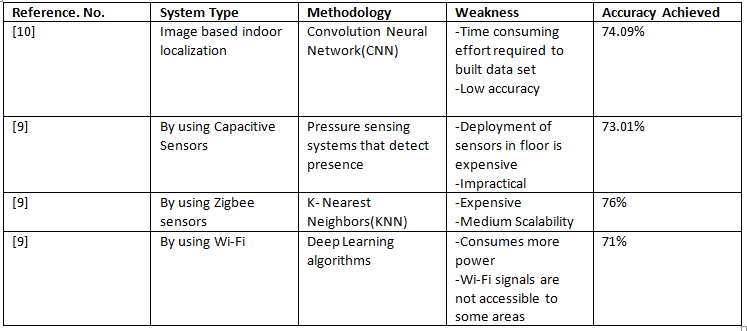
\includegraphics[scale=0.8]{abc}
\\Figure 1: Comparison of Existing Systems
\label{fig:five}
\end{center}





\subsection{Drawbacks of Existing Systems}
There are many drawbacks in existing systems. In some systems, camera is required for indoor positioning which is obtrusive for some users. High cost and effort is required for the deployment of indoor localization infrastructure. Most of the existing systems have medium or low accuracy. In image based indoor localization, time consuming effort is required for built data sets. Wi-Fi fingerprinting is relatively better than other systems because of finding position by using already deployed infrastructure. But its main drawback is that it consumes more power. There are some spots where Wi-Fi access points would be difficult to power. There are some areas where Wi-Fi signals are not accessible. In our proposed system, we will find indoor location using BLE beacons. BLE beacons are small in size, light weight and cheaper then Wi-Fi. BLE consumes less power than Wi-Fi. BLE beacons are usually battery powered, which are more flexible and easier deployed than sensors used by existing systems. BLE RSS signals can have a higher sample rate than Wi-Fi RSS signals (0.25 Hz~2 Hz). Our proposed system will provide more accuracy than existing systems and also it is unobtrusive. So, our proposed system will overcome the shortcomings in existing systems. Furthermore, our system will not only predict location but also provide information of that location and nearby location in form of text, videos, audio and images which is missing in existing systems because they find indoor positioning for different purposes\cite{zhuang2016smartphone}.

\section{Problem Statement}
Whenever a visitor goes to university campus or visits a new place, he does not know about the specifications of that area i.e. what happens in that specific room or what courses have been taught in a particular and its nearby labs. So, we are developing a system which assists them in determining the textual and pictorial information of a particular area and its nearby locations. For this purpose, we first find the indoor location of a user by using BLE beacons and RSSI values, and then provide information to him automatically on his android application. 
\section{Proposed System}
In our proposed system, an android application provide guidance to university visitors and make them familiar with university. Application will not only tell the current indoor location of user but also the information about current indoor location and nearby rooms in textual, image, audio or video form.
\\
Proposed system consist of these modules:
\heading{Deployment of BLE beacons}
BLE beacons will be deployed in the rooms. BLE beacons will be installed on the ceilings of rooms.
\heading{Data Acquisition}
BLE beacons broadcasts signals and these signals in the form of RSSI values will be captured at different positions by using android application and then csv file will be generated.
\heading{Data pre-processing and Training}
Data will be pre-processed and trained by using machine learning algorithm and then trained model will be deployed on server.
\heading{Room level prediction}
An android application for common users will be developed that capture RSSI signals and send to server. Then trained model will take these values as input for the purpose of prediction of room and then send back this information to application.
\heading{Information about location}
Application will fetch information data of current room and nearby rooms from server and then display these information to screen.
\\
\\
Here is the work flow of our project that gives basic idea about it:
\begin{center}
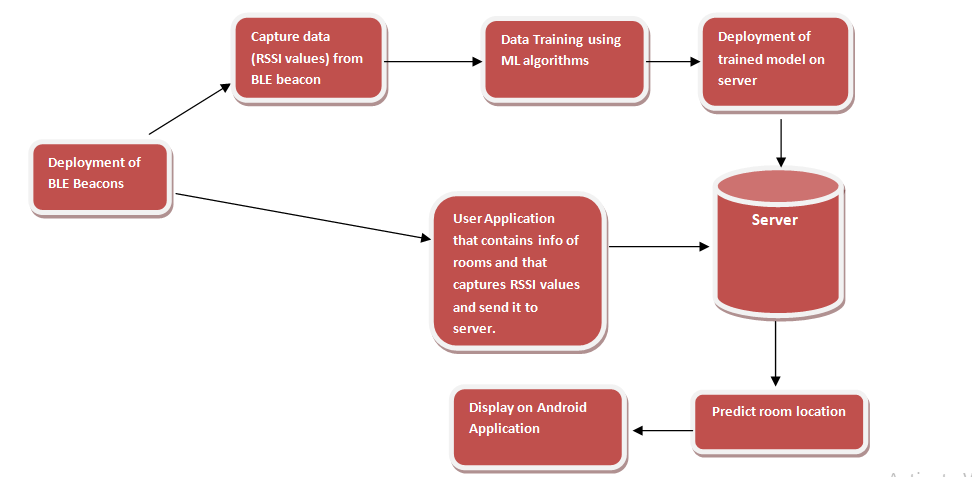
\includegraphics[scale=0.7]{diagram}
\\Figure 2: Work flow of project 
\end{center}

\section{Feasibility Study}


\subsection{Technical feasibility}
For the development of proposed system, we will use latest technologies. Android studio is used for development of android application. Weka API is used for machine learning. Weka is a machine learning library for Java. BLE beacons are used for capturing RSSI signals. BLE beacons are small in size, light weight, cheaper and easily available. Android application\cite{Localization} connects with BLE beacons through Bluetooth. BLE RSS signals can have a higher sample rate than Wi-Fi RSS signals (0.25 Hz~2 Hz). BLE beacons can easily deploy as compared to other sensors existing in market. We have necessary skill sets for the implementation of this project. This project requires understanding of machine learning, development of android application and understanding of how application communicate with BLE beacons and server. So, considering all these things, it is clear that our project is highly technical feasible and higher chances to be completed.
\subsection{Operational feasibility}
Operational feasibility means whether a proposed system is to be feasible at operational level. At user end, there is no additional hardware required. Users just need to install our android application on their smart phones which they easily get from play store. This application will guide the visitors of indoor building. In our case, visiting place will be CSE department. Students who do not familiar with campus rooms and activities are much likely to use this application. For this purpose, we conduct a market survey in order to know whether this project is acceptable for common people or not, 83.3 percent people find difficulty whenever they visit the place first time (see Figure 3). 58.3 percent people are interested in knowing their current indoor location and information related to it (see Figure 4). 91.7 percent people are interested in knowing the information of certain lab in textual as well as pictorial form on their mobile application (see Figure 5). 91.7 percent people think that this idea will bring ease to them (see Figure 6). This ensures the feasibility of our project at operational level.
\\
\\

\begin{center}
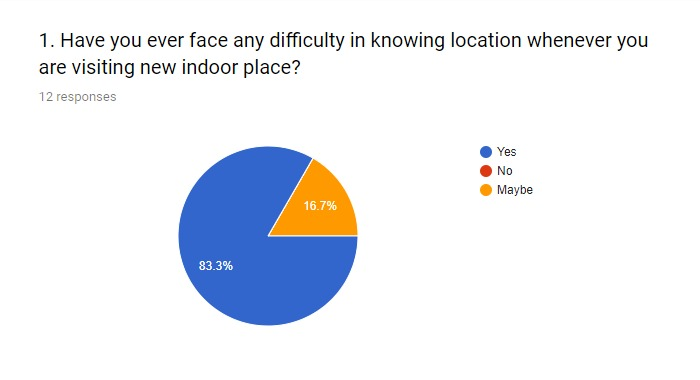
\includegraphics[scale=0.7]{graph1}
\\Figure 3: Problem
\end{center}


\begin{center}
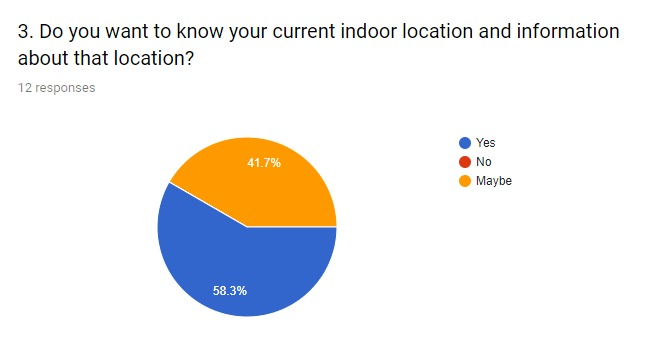
\includegraphics[scale=0.7]{graph3}
\\Figure 4: Indoor location
\end{center}

\begin{center}
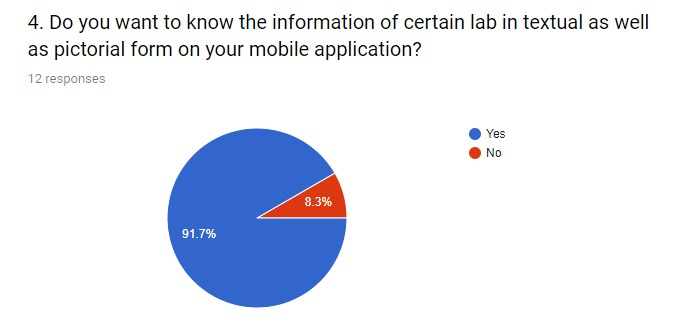
\includegraphics[scale=0.7]{graph4}
\\Figure 5: Information on Mobile Application
\end{center}

\begin{center}
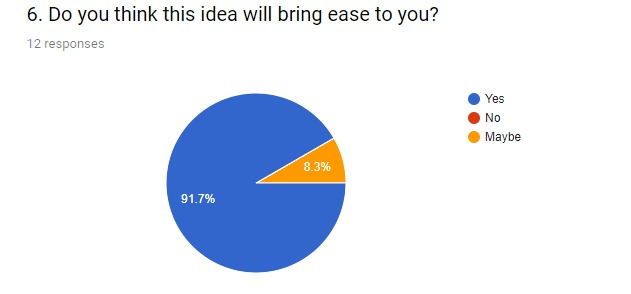
\includegraphics[scale=0.7]{graph6}
\\Figure 6: Bring Ease
\end{center}

 

\subsection{Economical feasibility}

Economical feasibility means whether a project is economically feasible by analyzing the cost required for developing and using this project. We will have to implement our proposed system in one department i.e. CSE dept. On average BLE beacons transmits signals upto 80 meters. So, we need almost 6 to 8 beacons which is sufficient for indoor localization in one department. The price of one BLE beacon ranges from 5 dollars to 30 dollars. Prices differ due to beacon signal range, typical battery life (which can be several years), and other factors. For deploying an android application on play store requires 25 dollars which is nearly equal to Rs 3,921. User doesn't need any cost for the installation of this application. For the purpose of machine learning we will use Weka API which is free and open source library. Android studio is used for development of application is also freely available. Only cost
involving factor is the purchasing of BLE beacons\cite{belmonte2017indoor} and publishing of Android application on play store. According to estimation, budget of this project is nearly Rs 8,601 which is affordable for us. So, this project is economically feasible.

\heading{Budget Plan}
\begin{center}
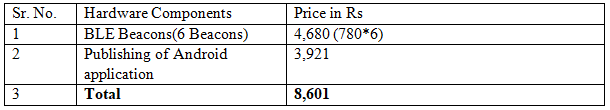
\includegraphics[scale=0.8]{table3}
\\Figure 7: Budget Plan
\end{center}
\section{System Requirements}
\subsection{Hardware Requirements}
\heading{Hardware requirements for Users}
Users just need a mobile device in which our application is installed.
\heading{Hardware requirements for Development}
\begin{center}
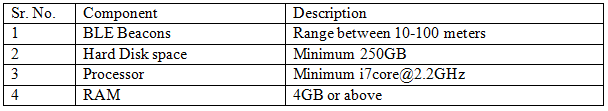
\includegraphics[scale=0.8]{table2}
\\Figure 8: Hardware Requirements
\end{center}
\subsection{Software Requirements}
\heading{Software Requirements for Users}
Installed android application and Bluetooth technology 

\heading{Software Requirements for Development}
\begin{center}
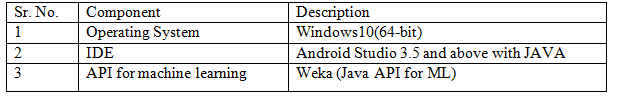
\includegraphics[scale=0.8]{table1}
\\Figure 9: Software Requirements
\end{center}


\section{Timeline of the project}
\begin{center}
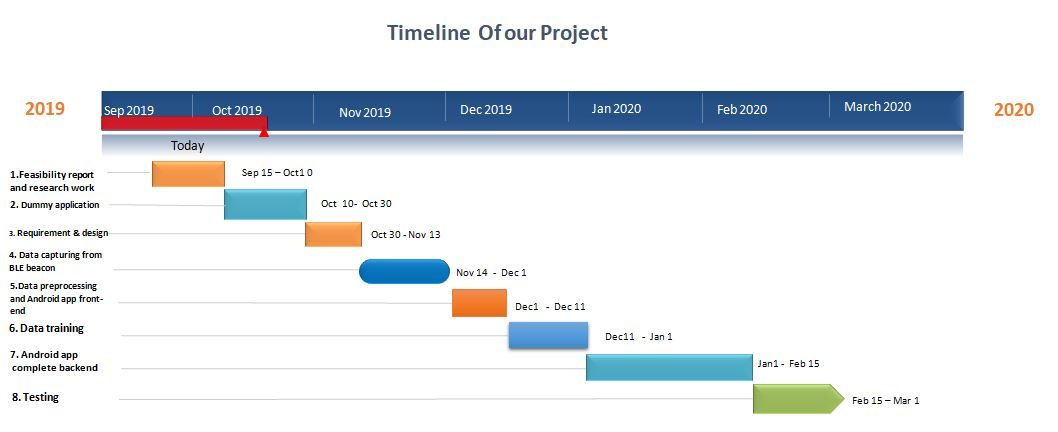
\includegraphics[scale=0.6]{timeline}
\\Figure 10: Timeline of the project
\end{center}
\section{Roles and activities of Team Members}
\begin{center}
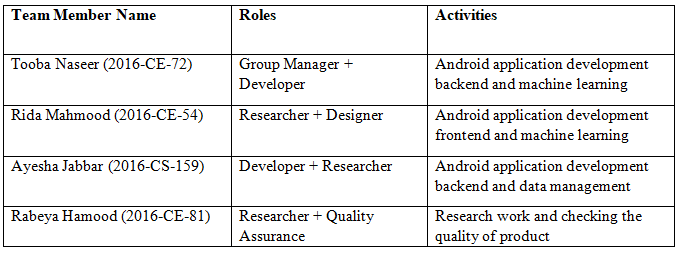
\includegraphics[scale=0.8]{table5}
\\Figure 11: Roles and activities of Team Members
\end{center}
\section{SWOT Analysis}
\subsection{Limitations and challenges}
\heading{Deployment of BLE beacons for indoor localization}
BLE beacons is used for collecting finger print such as RSSI value by mobile device. So, we will deploy BLE on different locations to access the finger print. To deploy the BLE beacons is big  challenge for us.
\heading{Using Android Studio}
Actually we are not familiar to android studio. We never worked on android studio before doing this project. So make the app development on android studio is also a big challenge for us. 
\heading{Send mobile app data to server}
To send data to the server is also a big challenge for us. Actually we get finger print from android app such as RSSI values. This data is converted into CSV file and sent to the server. We sent the data to the server by http protocol. 
\heading{Weka API is more compatible than MATLAB} 
For this purpose, we apply KNN algorithm on MATLAB or using Weka API. We conclude that to apply machine learning algorithm on Weka API is compatibility easier than MATLAB. So to select a right software is also a challenge for us. 
\heading{Send trained data to android application}
Actually, the purpose of this project is to guide the user about the place or nearby places where user is located. So after training the data, we sent the location of the person on android app in the form of text, video, image etc. To sent trained data in android app is also a big challenge for us. 
\heading{Limitations}
Here are some limitations of our project such as : 
\begin{itemize}
\item Installation of BLE beacons is required
\item Time consuming process
\item Handling only Android OS , other operating systems are not covered.
\item Availability of only 1 building for validating system.
\item Space constraints
\item Short range technology
\item To cover large area, more BLE beacons will be required.
\end{itemize}
\subsection{Strengths and Opportunities}

\heading{Strengths}
Here are some strengths of our project:
\begin{itemize}
\item Bluetooth beacons are much more compatible than Wi-Fi for indoor localization.
\item Android smart phones and tablets which occupy the major share in smart devices.
\item No special hardware installations required at user end.
\item It supports mobile devices such as  smart phones and tablets. 
\item Beacons are platform independent. 
\item Weka and Android studio is open source.
\end{itemize}
\heading{Opportunities}
Here are some Opportunities of our project:
\begin{itemize}
\item User can easily find the location where he stands.
\item Our app well-informed the user about that location.
\item It also tells to the user about nearby places.
\item User can know about the information which we provide in the form of text, video and images etc.
\end{itemize}
\pagebreak



\section{References}


\bibliographystyle{plain}
\bibliography{References}
\end{document}